\documentclass[12pt]{article}
\usepackage{geometry}
\geometry{margin=0.5in, bottom=0.35in, columnsep=1.0in}
\usepackage{graphicx, adjustbox, tikz-cd, amsmath, amssymb, multicol, lscape, mathtools}
%\usetikzlibrary{decorations.text}
%\usepackage{frcursive}\newcommand{\mathfrc}[1]{\text{\textcursive{#1}}}
\setlength{\parindent}{0pt} 
\begin{document}
\begin{landscape}
\pagestyle{empty}

%\sf
\huge 
Standard Normal %Cumulative Distribution Function $F_Z$ 
table

\vspace{0.2in}
\large
\hfill
\begin{tikzcd}[column sep=3.5cm, row sep=-2mm]
	\text{\LARGE standard units}\quad
	\rar[leftrightarrow, "\text{\normalsize use table to convert}"]
	& \quad\text{\LARGE percentile rank}
	\\ \displaystyle\boldsymbol z\color{black} = \frac{x-\mu}\sigma\quad\,\,
	& \quad\boldsymbol{P(z \text{ or less})}
	\color{black} = \text{area left of }z
	\end{tikzcd}
\hfill\hfill~
$\smash{\begin{matrix}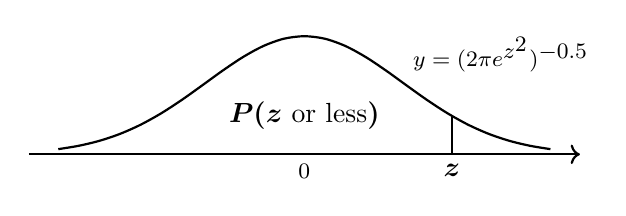
\begin{tikzpicture}[thick, yscale=1.5, xscale=1.25]
	\draw[smooth, domain=-2.5:2.5] plot (\x, {2.718^(-0.5*(\x*\x))});
	\draw (1, {2.718^-0.5}) node[above right, outer sep=0.4pt] (fZ) 
		{\footnotesize$\color{black} y=(2\pi e^{\textstyle z^{\textstyle2}})^{\textstyle-0.5}$};
	\draw (-2.8, 0) edge[->] (2.8, 0);
	\draw  (1.5,0) node[below] {$\boldsymbol z$} -- ++(up: {2.718^(-0.5*(1.5*1.5))});
	\draw (0,0) node[below, black, outer sep=0.4pt] {\footnotesize0};
	\draw (0, 0.33) node {$\boldsymbol{P(z\text{ or less})}$};
	\end{tikzpicture}\end{matrix}}$
\hfill~

% TO SHOW CLASS normal density function is a probability density function
% https://www.wolframalpha.com/input/?i=integrate+x*x*(2*pi*exp(x*x))%5E(-1%2F2)+from+negative+inf+to+inf

\footnotesize
%\begin{center}
\begin{adjustbox}{angle=270}
\def\arraystretch{0.68}
\begin{tabular}{
	r
	@{\hspace{4.5mm}}
	*{5}{c @{\hspace{2.5mm}}} 
	@{\hspace{-0.5mm}}
	*{5}{@{\hspace{2.5mm}} c} 
	@{\hspace{2mm}}
	r
	}
& 0.00 & 0.01 & 0.02 & 0.03 & 0.04 & 0.05 & 0.06 & 0.07 & 0.08 & 0.09 \\
&&&&&&&&&&{} \\
$\mathclap{\le\phantom\le}-$3.5$\mathclap{\phantom00}$ & 0.0001\\
$-$3.4 & 0.0003 & 0.0003 & 0.0003 & 0.0003 & 0.0003 & 0.0003 & 0.0003 & 0.0003 & 0.0003 & 0.0002 & $-$3.4 \\
$-$3.3 & 0.0005 & 0.0005 & 0.0005 & 0.0004 & 0.0004 & 0.0004 & 0.0004 & 0.0004 & 0.0004 & 0.0003 & $-$3.3 \\
$-$3.2 & 0.0007 & 0.0007 & 0.0006 & 0.0006 & 0.0006 & 0.0006 & 0.0006 & 0.0005 & 0.0005 & 0.0005 & $-$3.2 \\
$-$3.1 & 0.0010 & 0.0009 & 0.0009 & 0.0009 & 0.0008 & 0.0008 & 0.0008 & 0.0008 & 0.0007 & 0.0007 & $-$3.1 \\
$-$3.0 & 0.0013 & 0.0013 & 0.0013 & 0.0012 & 0.0012 & 0.0011 & 0.0011 & 0.0011 & 0.0010 & 0.0010 & $-$3.0 \\
&&&&&&&&&&{} \\
$-$2.9 & 0.0019 & 0.0018 & 0.0018 & 0.0017 & 0.0016 & 0.0016 & 0.0015 & 0.0015 & 0.0014 & 0.0014 & $-$2.9 \\
$-$2.8 & 0.0026 & 0.0025 & 0.0024 & 0.0023 & 0.0023 & 0.0022 & 0.0021 & 0.0021 & 0.0020 & 0.0019 & $-$2.8 \\
$-$2.7 & 0.0035 & 0.0034 & 0.0033 & 0.0032 & 0.0031 & 0.0030 & 0.0029 & 0.0028 & 0.0027 & 0.0026 & $-$2.7 \\
$-$2.6 & 0.0047 & 0.0045 & 0.0044 & 0.0043 & 0.0041 & 0.0040 & 0.0039 & 0.0038 & 0.0037 & 0.0036 & $-$2.6 \\
$-$2.5 & 0.0062 & 0.0060 & 0.0059 & 0.0057 & 0.0055 & 0.0054 & 0.0052 & 0.0051 & 0.0049 & 0.0048 & $-$2.5 \\
$-$2.4 & 0.0082 & 0.0080 & 0.0078 & 0.0075 & 0.0073 & 0.0071 & 0.0069 & 0.0068 & 0.0066 & 0.0064 & $-$2.4 \\
$-$2.3 & 0.0107 & 0.0104 & 0.0102 & 0.0099 & 0.0096 & 0.0094 & 0.0091 & 0.0089 & 0.0087 & 0.0084 & $-$2.3 \\
$-$2.2 & 0.0139 & 0.0136 & 0.0132 & 0.0129 & 0.0125 & 0.0122 & 0.0119 & 0.0116 & 0.0113 & 0.0110 & $-$2.2 \\
$-$2.1 & 0.0179 & 0.0174 & 0.0170 & 0.0166 & 0.0162 & 0.0158 & 0.0154 & 0.0150 & 0.0146 & 0.0143 & $-$2.1 \\
$-$2.0 & 0.0228 & 0.0222 & 0.0217 & 0.0212 & 0.0207 & 0.0202 & 0.0197 & 0.0192 & 0.0188 & 0.0183 & $-$2.0 \\
&&&&&&&&&&{} \\
$-$1.9 & 0.0287 & 0.0281 & 0.0274 & 0.0268 & 0.0262 & 0.0256 & 0.0250 & 0.0244 & 0.0239 & 0.0233 & $-$1.9 \\
$-$1.8 & 0.0359 & 0.0351 & 0.0344 & 0.0336 & 0.0329 & 0.0322 & 0.0314 & 0.0307 & 0.0301 & 0.0294 & $-$1.8 \\
$-$1.7 & 0.0446 & 0.0436 & 0.0427 & 0.0418 & 0.0409 & 0.0401 & 0.0392 & 0.0384 & 0.0375 & 0.0367 & $-$1.7 \\
$-$1.6 & 0.0548 & 0.0537 & 0.0526 & 0.0516 & 0.0505 & 0.0495 & 0.0485 & 0.0475 & 0.0465 & 0.0455 & $-$1.6 \\
$-$1.5 & 0.0668 & 0.0655 & 0.0643 & 0.0630 & 0.0618 & 0.0606 & 0.0594 & 0.0582 & 0.0571 & 0.0559 & $-$1.5 \\
$-$1.4 & 0.0808 & 0.0793 & 0.0778 & 0.0764 & 0.0749 & 0.0735 & 0.0721 & 0.0708 & 0.0694 & 0.0681 & $-$1.4 \\
$-$1.3 & 0.0968 & 0.0951 & 0.0934 & 0.0918 & 0.0901 & 0.0885 & 0.0869 & 0.0853 & 0.0838 & 0.0823 & $-$1.3 \\
$-$1.2 & 0.1151 & 0.1131 & 0.1112 & 0.1093 & 0.1075 & 0.1057 & 0.1038 & 0.1020 & 0.1003 & 0.0985 & $-$1.2 \\
$-$1.1 & 0.1357 & 0.1335 & 0.1314 & 0.1292 & 0.1271 & 0.1251 & 0.1230 & 0.1210 & 0.1190 & 0.1170 & $-$1.1 \\
$-$1.0 & 0.1587 & 0.1562 & 0.1539 & 0.1515 & 0.1492 & 0.1469 & 0.1446 & 0.1423 & 0.1401 & 0.1379 & $-$1.0 \\
&&&&&&&&&&{} \\
$-$0.9 & 0.1841 & 0.1814 & 0.1788 & 0.1762 & 0.1736 & 0.1711 & 0.1685 & 0.1660 & 0.1635 & 0.1611 & $-$0.9 \\
$-$0.8 & 0.2119 & 0.2090 & 0.2061 & 0.2033 & 0.2005 & 0.1977 & 0.1949 & 0.1922 & 0.1894 & 0.1867 & $-$0.8 \\
$-$0.7 & 0.2420 & 0.2389 & 0.2358 & 0.2327 & 0.2297 & 0.2266 & 0.2236 & 0.2207 & 0.2177 & 0.2148 & $-$0.7 \\
$-$0.6 & 0.2743 & 0.2709 & 0.2676 & 0.2643 & 0.2611 & 0.2578 & 0.2546 & 0.2514 & 0.2483 & 0.2451 & $-$0.6 \\
$-$0.5 & 0.3085 & 0.3050 & 0.3015 & 0.2981 & 0.2946 & 0.2912 & 0.2877 & 0.2843 & 0.2810 & 0.2776 & $-$0.5 \\
$-$0.4 & 0.3446 & 0.3409 & 0.3372 & 0.3336 & 0.3300 & 0.3264 & 0.3228 & 0.3192 & 0.3156 & 0.3121 & $-$0.4 \\
$-$0.3 & 0.3821 & 0.3783 & 0.3745 & 0.3707 & 0.3669 & 0.3632 & 0.3594 & 0.3557 & 0.3520 & 0.3483 & $-$0.3 \\
$-$0.2 & 0.4207 & 0.4168 & 0.4129 & 0.4090 & 0.4052 & 0.4013 & 0.3974 & 0.3936 & 0.3897 & 0.3859 & $-$0.2 \\
$-$0.1 & 0.4602 & 0.4562 & 0.4522 & 0.4483 & 0.4443 & 0.4404 & 0.4364 & 0.4325 & 0.4286 & 0.4247 & $-$0.1 \\
$-$0.0 & 0.5000 & 0.4960 & 0.4920 & 0.4880 & 0.4840 & 0.4801 & 0.4761 & 0.4721 & 0.4681 & 0.4641 & $-$0.0 \\
&&&&&&&&&&{} \\
0.0 & 0.5000 & 0.5040 & 0.5080 & 0.5120 & 0.5160 & 0.5199 & 0.5239 & 0.5279 & 0.5319 & 0.5359 & 0.0 \\
0.1 & 0.5398 & 0.5438 & 0.5478 & 0.5517 & 0.5557 & 0.5596 & 0.5636 & 0.5675 & 0.5714 & 0.5753 & 0.1 \\
0.2 & 0.5793 & 0.5832 & 0.5871 & 0.5910 & 0.5948 & 0.5987 & 0.6026 & 0.6064 & 0.6103 & 0.6141 & 0.2 \\
0.3 & 0.6179 & 0.6217 & 0.6255 & 0.6293 & 0.6331 & 0.6368 & 0.6406 & 0.6443 & 0.6480 & 0.6517 & 0.3 \\
0.4 & 0.6554 & 0.6591 & 0.6628 & 0.6664 & 0.6700 & 0.6736 & 0.6772 & 0.6808 & 0.6844 & 0.6879 & 0.4 \\
0.5 & 0.6915 & 0.6950 & 0.6985 & 0.7019 & 0.7054 & 0.7088 & 0.7123 & 0.7157 & 0.7190 & 0.7224 & 0.5 \\
0.6 & 0.7257 & 0.7291 & 0.7324 & 0.7357 & 0.7389 & 0.7422 & 0.7454 & 0.7486 & 0.7517 & 0.7549 & 0.6 \\
0.7 & 0.7580 & 0.7611 & 0.7642 & 0.7673 & 0.7704 & 0.7734 & 0.7764 & 0.7794 & 0.7823 & 0.7852 & 0.7 \\
0.8 & 0.7881 & 0.7910 & 0.7939 & 0.7967 & 0.7995 & 0.8023 & 0.8051 & 0.8079 & 0.8106 & 0.8133 & 0.8 \\
0.9 & 0.8159 & 0.8186 & 0.8212 & 0.8238 & 0.8264 & 0.8289 & 0.8315 & 0.8340 & 0.8365 & 0.8389 & 0.9 \\
&&&&&&&&&&{} \\
1.0 & 0.8413 & 0.8438 & 0.8461 & 0.8485 & 0.8508 & 0.8531 & 0.8554 & 0.8577 & 0.8599 & 0.8621 & 1.0 \\
1.1 & 0.8643 & 0.8665 & 0.8686 & 0.8708 & 0.8729 & 0.8749 & 0.8770 & 0.8790 & 0.8810 & 0.8830 & 1.1 \\
1.2 & 0.8849 & 0.8869 & 0.8888 & 0.8907 & 0.8925 & 0.8944 & 0.8962 & 0.8980 & 0.8997 & 0.9015 & 1.2 \\
1.3 & 0.9032 & 0.9049 & 0.9066 & 0.9082 & 0.9099 & 0.9115 & 0.9131 & 0.9147 & 0.9162 & 0.9177 & 1.3 \\
1.4 & 0.9192 & 0.9207 & 0.9222 & 0.9236 & 0.9251 & 0.9265 & 0.9279 & 0.9292 & 0.9306 & 0.9319 & 1.4 \\
1.5 & 0.9332 & 0.9345 & 0.9357 & 0.9370 & 0.9382 & 0.9394 & 0.9406 & 0.9418 & 0.9429 & 0.9441 & 1.5 \\
1.6 & 0.9452 & 0.9463 & 0.9474 & 0.9484 & 0.9495 & 0.9505 & 0.9515 & 0.9525 & 0.9535 & 0.9545 & 1.6 \\
1.7 & 0.9554 & 0.9564 & 0.9573 & 0.9582 & 0.9591 & 0.9599 & 0.9608 & 0.9616 & 0.9625 & 0.9633 & 1.7 \\
1.8 & 0.9641 & 0.9649 & 0.9656 & 0.9664 & 0.9671 & 0.9678 & 0.9686 & 0.9693 & 0.9699 & 0.9706 & 1.8 \\
1.9 & 0.9713 & 0.9719 & 0.9726 & 0.9732 & 0.9738 & 0.9744 & 0.9750 & 0.9756 & 0.9761 & 0.9767 & 1.9 \\
&&&&&&&&&&{} \\
2.0 & 0.9773 & 0.9778 & 0.9783 & 0.9788 & 0.9793 & 0.9798 & 0.9803 & 0.9808 & 0.9812 & 0.9817 & 2.0 \\
2.1 & 0.9821 & 0.9826 & 0.9830 & 0.9834 & 0.9838 & 0.9842 & 0.9846 & 0.9850 & 0.9854 & 0.9857 & 2.1 \\
2.2 & 0.9861 & 0.9864 & 0.9868 & 0.9871 & 0.9875 & 0.9878 & 0.9881 & 0.9884 & 0.9887 & 0.9890 & 2.2 \\
2.3 & 0.9893 & 0.9896 & 0.9898 & 0.9901 & 0.9904 & 0.9906 & 0.9909 & 0.9911 & 0.9913 & 0.9916 & 2.3 \\
2.4 & 0.9918 & 0.9920 & 0.9922 & 0.9925 & 0.9927 & 0.9929 & 0.9931 & 0.9932 & 0.9934 & 0.9936 & 2.4 \\
2.5 & 0.9938 & 0.9940 & 0.9941 & 0.9943 & 0.9945 & 0.9946 & 0.9948 & 0.9949 & 0.9951 & 0.9952 & 2.5 \\
2.6 & 0.9953 & 0.9955 & 0.9956 & 0.9957 & 0.9959 & 0.9960 & 0.9961 & 0.9962 & 0.9963 & 0.9964 & 2.6 \\
2.7 & 0.9965 & 0.9966 & 0.9967 & 0.9968 & 0.9969 & 0.9970 & 0.9971 & 0.9972 & 0.9973 & 0.9974 & 2.7 \\
2.8 & 0.9974 & 0.9975 & 0.9976 & 0.9977 & 0.9977 & 0.9978 & 0.9979 & 0.9979 & 0.9980 & 0.9981 & 2.8 \\
2.9 & 0.9981 & 0.9982 & 0.9983 & 0.9983 & 0.9984 & 0.9984 & 0.9985 & 0.9985 & 0.9986 & 0.9986 & 2.9 \\
&&&&&&&&&&{} \\
3.0 & 0.9987 & 0.9987 & 0.9987 & 0.9988 & 0.9988 & 0.9989 & 0.9989 & 0.9989 & 0.9990 & 0.9990 & 3.0 \\
3.1 & 0.9990 & 0.9991 & 0.9991 & 0.9991 & 0.9992 & 0.9992 & 0.9992 & 0.9992 & 0.9993 & 0.9993 & 3.1 \\
3.2 & 0.9993 & 0.9993 & 0.9994 & 0.9994 & 0.9994 & 0.9994 & 0.9994 & 0.9995 & 0.9995 & 0.9995 & 3.2 \\
3.3 & 0.9995 & 0.9995 & 0.9995 & 0.9996 & 0.9996 & 0.9996 & 0.9996 & 0.9996 & 0.9996 & 0.9997 & 3.3 \\
3.4 & 0.9997 & 0.9997 & 0.9997 & 0.9997 & 0.9997 & 0.9997 & 0.9997 & 0.9997 & 0.9997 & 0.9998 & 3.4 \\
$\mathclap{\ge\phantom\ge}$3.5$\mathclap{\phantom00}$ & 0.0001\\
&&&&&&&&&&{} \\
& 0.00 & 0.01 & 0.02 & 0.03 & 0.04 & 0.05 & 0.06 & 0.07 & 0.08 & 0.09
\end{tabular}
\end{adjustbox}
%\end{center}
\par\vfill\small
City University of New York / College of Staten Island / M Sunderland
\hfill
\textcolor{black}{symmetry: $P(-z$ or less) = $1 - P(z$ or less)}
\end{landscape}

\pagestyle{empty}
\begin{landscape}
\huge 
Student's $t$ table
\par\vfill
\begin{adjustbox}{angle=270}
\normalsize
\def\arraystretch{0.82}
\begin{tabular}{r@{\qquad}rrrrr@{\qquad}r}
{} & $\smash{\alpha_{\textstyle\phantom{\!/\!2}}}$ 
= 0.0100 & 0.0200 & 0.0500 & 0.1000 & 0.2000 & {} \\[3ex]
df = 1 & $\smash{t_{\textstyle\alpha\!/\!2}}$ 
= $\phantom0$63.66 & 31.82 & 12.71 & 6.31 & 3.08 & df = 1 \\
2 & 9.92 & 6.96 & 4.30 & 2.92 & 1.89 & 2 \\
3 & 5.84 & 4.54 & 3.18 & 2.35 & 1.64 & 3 \\
4 & 4.60 & 3.75 & 2.78 & 2.13 & 1.53 & 4 \\
5 & 4.03 & 3.36 & 2.57 & 2.02 & 1.48 & 5 \\
6 & 3.71 & 3.14 & 2.45 & 1.94 & 1.44 & 6 \\
7 & 3.50 & 3.00 & 2.36 & 1.89 & 1.41 & 7 \\
8 & 3.36 & 2.90 & 2.31 & 1.86 & 1.40 & 8 \\
9 & 3.25 & 2.82 & 2.26 & 1.83 & 1.38 & 9 \\[2.5ex]
10 & 3.17 & 2.76 & 2.23 & 1.81 & 1.37 & 10 \\
11 & 3.11 & 2.72 & 2.20 & 1.80 & 1.36 & 11 \\
12 & 3.05 & 2.68 & 2.18 & 1.78 & 1.36 & 12 \\
13 & 3.01 & 2.65 & 2.16 & 1.77 & 1.35 & 13 \\
14 & 2.98 & 2.62 & 2.14 & 1.76 & 1.35 & 14 \\
15 & 2.95 & 2.60 & 2.13 & 1.75 & 1.34 & 15 \\
16 & 2.92 & 2.58 & 2.12 & 1.75 & 1.34 & 16 \\
17 & 2.90 & 2.57 & 2.11 & 1.74 & 1.33 & 17 \\
18 & 2.88 & 2.55 & 2.10 & 1.73 & 1.33 & 18 \\
19 & 2.86 & 2.54 & 2.09 & 1.73 & 1.33 & 19 \\[2.5ex]
20 & 2.85 & 2.53 & 2.09 & 1.72 & 1.33 & 20 \\
21 & 2.83 & 2.52 & 2.08 & 1.72 & 1.32 & 21 \\
22 & 2.82 & 2.51 & 2.07 & 1.72 & 1.32 & 22 \\
23 & 2.81 & 2.50 & 2.07 & 1.71 & 1.32 & 23 \\
24 & 2.80 & 2.49 & 2.06 & 1.71 & 1.32 & 24 \\
25 & 2.79 & 2.49 & 2.06 & 1.71 & 1.32 & 25 \\
26 & 2.78 & 2.48 & 2.06 & 1.71 & 1.31 & 26 \\
27 & 2.77 & 2.47 & 2.05 & 1.70 & 1.31 & 27 \\
28 & 2.76 & 2.47 & 2.05 & 1.70 & 1.31 & 28 \\
29 & 2.76 & 2.46 & 2.05 & 1.70 & 1.31 & 29 \\[2.5ex]
30 & 2.75 & 2.46 & 2.04 & 1.70 & 1.31 & 30 \\
31 & 2.74 & 2.45 & 2.04 & 1.70 & 1.31 & 31 \\
32 & 2.74 & 2.45 & 2.04 & 1.69 & 1.31 & 32 \\
33 & 2.73 & 2.44 & 2.03 & 1.69 & 1.31 & 33 \\
34 & 2.73 & 2.44 & 2.03 & 1.69 & 1.31 & 34 \\
35 & 2.72 & 2.44 & 2.03 & 1.69 & 1.31 & 35 \\
36 & 2.72 & 2.43 & 2.03 & 1.69 & 1.31 & 36 \\
37 & 2.72 & 2.43 & 2.03 & 1.69 & 1.30 & 37 \\
38 & 2.71 & 2.43 & 2.02 & 1.69 & 1.30 & 38 \\
39 & 2.71 & 2.43 & 2.02 & 1.68 & 1.30 & 39 \\[2.5ex]
40 & 2.70 & 2.42 & 2.02 & 1.68 & 1.30 & 40 \\
45 & 2.69 & 2.41 & 2.01 & 1.68 & 1.30 & 45 \\
50 & 2.68 & 2.40 & 2.01 & 1.68 & 1.30 & 50 \\
60 & 2.66 & 2.39 & 2.00 & 1.67 & 1.30 & 60 \\
70 & 2.65 & 2.38 & 1.99 & 1.67 & 1.29 & 70 \\
80 & 2.64 & 2.37 & 1.99 & 1.66 & 1.29 & 80 \\
90 & 2.63 & 2.37 & 1.99 & 1.66 & 1.29 & 90 \\[2.5ex]
100 & 2.63 & 2.36 & 1.98 & 1.66 & 1.29 & 100 \\
200 & 2.60 & 2.35 & 1.97 & 1.65 & 1.29 & 200 \\
300 & 2.59 & 2.34 & 1.97 & 1.65 & 1.28 & 300 \\
400 & 2.59 & 2.34 & 1.97 & 1.65 & 1.28 & 400 \\
500 & 2.59 & 2.33 & 1.96 & 1.65 & 1.28 & 500 \\
$\ge$600 & 2.58 & 2.33 & 1.96 & 1.65 & 1.28 & $\ge$600 \\[3ex]
{} & $\smash{\alpha_{\textstyle\phantom{\!/\!2}}}$ 
= 0.0100 & 0.0200 & 0.0500 & 0.1000 & 0.2000 & {} 
\end{tabular}
\end{adjustbox}
\par\vfill\vfill\small
City University of New York / College of Staten Island / M Sunderland
\end{landscape}

\newcommand\halftable{
	\huge 
	$F_Z$ table
	\par\bigskip\bigskip\footnotesize
	\begin{tabular}{
			r 
			| *{5}{c @{\hspace{1.2mm}}} 
			|
			*{5}{@{\hspace{1.2mm}} c} 
			| l
			}
		& 0.00 & 0.01 & 0.02 & 0.03 & 0.04 & 0.05 & 0.06 & 0.07 & 0.08 & 0.09 \\ \hline 
		0.0 & .5000 & .5040 & .5080 & .5120 & .5160 & .5199 & .5239 & .5279 & .5319 & .5359 & 0.0 \\
		0.1 & .5398 & .5438 & .5478 & .5517 & .5557 & .5596 & .5636 & .5675 & .5714 & .5753 & 0.1 \\
		0.2 & .5793 & .5832 & .5871 & .5910 & .5948 & .5987 & .6026 & .6064 & .6103 & .6141 & 0.2 \\
		0.3 & .6179 & .6217 & .6255 & .6293 & .6331 & .6368 & .6406 & .6443 & .6480 & .6517 & 0.3 \\
		0.4 & .6554 & .6591 & .6628 & .6664 & .6700 & .6736 & .6772 & .6808 & .6844 & .6879 & 0.4 \\
		0.5 & .6915 & .6950 & .6985 & .7019 & .7054 & .7088 & .7123 & .7157 & .7190 & .7224 & 0.5 \\
		0.6 & .7257 & .7291 & .7324 & .7357 & .7389 & .7422 & .7454 & .7486 & .7517 & .7549 & 0.6 \\
		0.7 & .7580 & .7611 & .7642 & .7673 & .7704 & .7734 & .7764 & .7794 & .7823 & .7852 & 0.7 \\
		0.8 & .7881 & .7910 & .7939 & .7967 & .7995 & .8023 & .8051 & .8079 & .8106 & .8133 & 0.8 \\
		0.9 & .8159 & .8186 & .8212 & .8238 & .8264 & .8289 & .8315 & .8340 & .8365 & .8389 & 0.9 \\ \hline
		1.0 & .8413 & .8438 & .8461 & .8485 & .8508 & .8531 & .8554 & .8577 & .8599 & .8621 & 1.0 \\
		1.1 & .8643 & .8665 & .8686 & .8708 & .8729 & .8749 & .8770 & .8790 & .8810 & .8830 & 1.1 \\
		1.2 & .8849 & .8869 & .8888 & .8907 & .8925 & .8944 & .8962 & .8980 & .8997 & .9015 & 1.2 \\
		1.3 & .9032 & .9049 & .9066 & .9082 & .9099 & .9115 & .9131 & .9147 & .9162 & .9177 & 1.3 \\
		1.4 & .9192 & .9207 & .9222 & .9236 & .9251 & .9265 & .9279 & .9292 & .9306 & .9319 & 1.4 \\
		1.5 & .9332 & .9345 & .9357 & .9370 & .9382 & .9394 & .9406 & .9418 & .9429 & .9441 & 1.5 \\
		1.6 & .9452 & .9463 & .9474 & .9484 & .9495 & .9505 & .9515 & .9525 & .9535 & .9545 & 1.6 \\
		1.7 & .9554 & .9564 & .9573 & .9582 & .9591 & .9599 & .9608 & .9616 & .9625 & .9633 & 1.7 \\
		1.8 & .9641 & .9649 & .9656 & .9664 & .9671 & .9678 & .9686 & .9693 & .9699 & .9706 & 1.8 \\
		1.9 & .9713 & .9719 & .9726 & .9732 & .9738 & .9744 & .9750 & .9756 & .9761 & .9767 & 1.9 \\ \hline
		2.0 & .9773 & .9778 & .9783 & .9788 & .9793 & .9798 & .9803 & .9808 & .9812 & .9817 & 2.0 \\
		2.1 & .9821 & .9826 & .9830 & .9834 & .9838 & .9842 & .9846 & .9850 & .9854 & .9857 & 2.1 \\
		2.2 & .9861 & .9864 & .9868 & .9871 & .9875 & .9878 & .9881 & .9884 & .9887 & .9890 & 2.2 \\
		2.3 & .9893 & .9896 & .9898 & .9901 & .9904 & .9906 & .9909 & .9911 & .9913 & .9916 & 2.3 \\
		2.4 & .9918 & .9920 & .9922 & .9925 & .9927 & .9929 & .9931 & .9932 & .9934 & .9936 & 2.4 \\
		2.5 & .9938 & .9940 & .9941 & .9943 & .9945 & .9946 & .9948 & .9949 & .9951 & .9952 & 2.5 \\
		2.6 & .9953 & .9955 & .9956 & .9957 & .9959 & .9960 & .9961 & .9962 & .9963 & .9964 & 2.6 \\
		2.7 & .9965 & .9966 & .9967 & .9968 & .9969 & .9970 & .9971 & .9972 & .9973 & .9974 & 2.7 \\
		2.8 & .9974 & .9975 & .9976 & .9977 & .9977 & .9978 & .9979 & .9979 & .9980 & .9981 & 2.8 \\
		2.9 & .9981 & .9982 & .9983 & .9983 & .9984 & .9984 & .9985 & .9985 & .9986 & .9986 & 2.9 \\ 
		3.0 & .9987 & .9987 & .9987 & .9988 & .9988 & .9989 & .9989 & .9989 & .9990 & .9990 & 3.0 \\ \hline
		& 0.00 & 0.01 & 0.02 & 0.03 & 0.04 & 0.05 & 0.06 & 0.07 & 0.08 & 0.09
		\end{tabular}
	}

\begin{landscape}
\begin{multicols}2
	\def\arraystretch{1.25}
	\center\par\halftable
	\par\halftable
	\end{multicols}

\begin{multicols}2
	\def\arraystretch{1.25}
	\center\par\halftable
	\par\halftable
	\end{multicols}
	\end{landscape}
\end{document}


# TO GENERATE TABLES (python)
from scipy.stats import norm, t
Phi = norm.cdf
F_t = t.cdf
for z1 in (0.1*i for i in range(-34,1)):
	print('$-$%.1f' % abs(z1), end='')
	for z2 in (0.01*i for i in range(10)):
		print(' & %.4f' % Phi(z1+z2), end='')
	print(' & $-$%.1f \\\\' % abs(z1))

for z1 in (0.1*i for i in range(35)):
	print('%.1f' % z1, end='')
	for z2 in (0.01*i for i in range(10)):
		print(' & %.4f' % Phi(z1+z2), end='')
	print(' & %.1f \\\\' % z1)

for df in list(range(1,41)) + [45,50,60,70,80,90,100,200,300,400,500,600,1000,2000,10000]:
	print(df, end="")
	for a in [0.01, 0.02, 0.05, 0.10, 0.20]:
		t = round(-1*Finv_t(a/2, df), 2)
		if t*10%1 == 0: addzero = "0"
		else: addzero = ""
		t = str(t) + addzero
		print(" & " + t, end="")
	print(" & " + str(df), end="")
	print(" \\\\")